\section{Manipulation 5 "Déterminer expérimentalement l'évolution du
module de Young en fonction de la température pour au moins un
matériau."}
\subsection{Approches / Méthodes}
\subsubsection{\large Rappels Théoriques}
\paragraph{Introduction}
    Après avoir mesuré la vitesse du son dans différents matériaux et
    calculé leur module de Young, nous nous intéressons maintenant à
    l'impact de la température sur ces mesures.
\paragraph{Equations physiques}
    Nous cherchons à exprimer le module de Young du matériau en fonction
    de la température à laquelle se trouve l'objet. Ceci dans le but
    d'évaluer l'influence de la température sur l'élasticité du matériau.
    ~\cite{Polycop-Ondes}
\begin{align}
    \intertext{
    Pour faire ceci nous allons utiliser la formule de la célérité du son
    utilisée l'équation 14}
    c &= \sqrt[]{\frac{E}{\rho}} => E = \rho c^2
    \intertext{Utilisons la formule de la dilatation volumique et les
    définitions de la masse volumique, du $\Delta \theta$ et du volume
    d'un cylindre :}
    V &= V_0(1+3\alpha \Delta \theta); V_0 = L_0 \frac{D_0^2\pi}{4};
    \rho = \frac{m}{V};\Delta \theta=\theta_f-\theta_i
    \intertext{Finalement on obtient :}
    E(\theta_f) &= \frac{4mc^2}{L_0D_0^2\pi\left(1+3\alpha(\theta_f-
    \theta_i)\right)}
\end{align}

Dans cette formule on a besoin de 5 paramètres fixes dépendants de notre
objet, soit la longueur initiale $L_0$ [m], le diamètre initial de notre
barre $D_0$ [m], sa masse $m$ [kg], le coefficient de dilatation linéique
du matériau $\alpha$ [1/°C] et la température à laquelle ont été mesurées
les dimensions initiales $\theta_i$ [°C].\\

Deux autres paramètres sont interdépendants : la température de l'objet
$\theta_f$ et la célérité du son mesurée $c$ [m/s] au moment de la
mesure.\\

Le résultat sera le module d'élasticité $E$ [GPa] du matériau à la
température $\theta_f$.\\

Pour les mesures de températures, nous avons décider d'utiliser les °C et
non les °K. En effet, l'unité d'un delta de température n'a pas
d'importance (Kelvin ou Celsius).
\paragraph{Calculs d'incertitudes}
    Selon la loi de propagations des incertitudes, nous pouvons en déduire
    l'erreur absolue sur le module de Young~\cite{gravier-laurent} :
    \begin{align}
    dE &= E \left(\frac{dm}{m}+2\frac{dc}{c}+\frac{\frac{dL_0}{L_0}+
    2\frac{dD_0}{D_0}+\left(\frac{dL_0}{L_0}+2\frac{dD_0}{D_0}+\frac{d
    \alpha}{\alpha}+\frac{d\theta_f+d\theta_i}{\theta_f-\theta_i}\right)
    \alpha(\theta_f-\theta_i)}{1+3\alpha (\theta_f-\theta_i)}\right)
    \end{align}
\subsubsection{\large Protocole expérimental}
    Cette expérience est un complément aux expériences précédentes. L'objet est
    chauffé uniformément en étant plongé dans un récipient d'eau
    chauffée avec une plaque chauffante. Lorsque celui-ci aura atteint la
    température voulue, nous le sortirons de l'eau. À partir de ce
    moment-là nous effectuerons des mesures régulières de la température
    au fur-et-à-mesure que celle-ci descend et de la célérité du son qui
    le traverse. 
\paragraph{Montage}

\begin{figure}[h]
    \centering
    \adjustbox{max width=\textwidth}{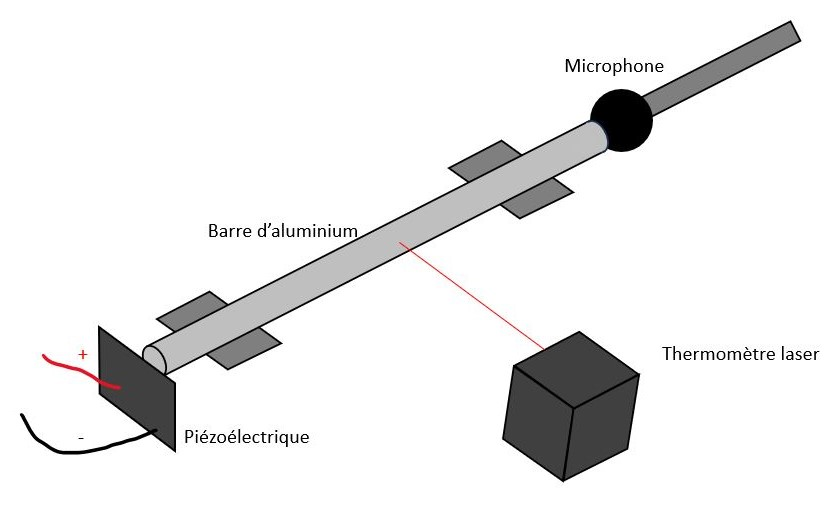
\includegraphics{montage_5.png}}
    \caption{Montage expérimental manipulation n°5}
\end{figure}
\newpage
\paragraph{Liste du matériel}
Le matériel utilisé est le même que 
celui de la première manipulation, 
avec l'ajout du matériel suivant pour 
effectuer les mesures :
\begin{itemize}
    \item Tige en aluminium, de longueur 100 mm et de diamètre 10 mm.\\
    \item Tige en acier inox, de longueur 100 mm et de diamètre 10 mm.\\
    \item Plaque chauffante\\
    \item Récipient chauffable\\
    \item Thermomètre laser\\
\end{itemize}

\paragraph{Méthode de mesure}
    Pour effectuer les mesures, il sera nécessaire d'avoir le moins
    de contact possible avec le matériau pour garder une température
    homogène. Pour faire ceci, nous allons utiliser un thermomètre laser.\\
    Faire des mesures sur un objet à une température homogène fixe
    ($\neq$ température de la salle) n'est pas facile, parce que celui-ci
    va vouloir tendre vers la température ambiante. Nous allons donc
    effectuer une série de mesures de température et de la célérité des
    vibrations d'une température proche de 100°C à une température
    approchant 20°C (idéalement entre 20 et 30 mesures). Ces mesures seront
    entrées dans un tableau Excel qui tracera la courbe de variation du
    module de Young.


\newpage

\subsection{\large Résultats / Analyse}
\subsubsection{\large Données brutes}
\paragraph{\large Cylindre Aluminium 100 mm}
\paragraph{Tableau}
\paragraph{Graphe}
\paragraph{Observations}

\paragraph{\large Cylindre Acier inox 100 mm}
\paragraph{Tableau}
\paragraph{Graphe}
\paragraph{Observations}

\newpage

\subsubsection{\large Données réduites}
\paragraph{\large Cylindre Aluminium 100 mm}
\paragraph{Calculs}
\paragraph{Incertitudes}
\paragraph{Régression Linéaire}

\paragraph{\large Cylindre Acier inox 100 mm}
\paragraph{Calculs}
\paragraph{Incertitudes}
\paragraph{Régression Linéaire}
\newpage

\subsubsection{\large Tableau récapitulatif}
\paragraph{Valeurs}
\paragraph{Incertitudes relatives}
\paragraph{Ecart relatif}

\subsubsection{\large Discussion quantitative}
\paragraph{Incertitude > écart}
validation
\paragraph{Incertitude < écart}
invalidation
discussion critique des méthodes